\providecommand{\canorm}[1]{\mathopen{{}^{\circ}_{\circ}}#1\mathclose{{}^{\circ}_{\circ}}}
\subsectionlink{Virasoro 代数}
\label{sec:2.6}

この章ではここまで、2次元の場の理論の局所的な性質を調べてきた。ここからは理論のスペクトルに関心を移す。空間座標は閉弦の場合のように周期的であるか、開弦の場合のように有界であるものとする。

周期的な場合には、
\begin{equation}
\sigma^1\sim\sigma^1+2\pi.
\tag{2.6.1}\label{eq:2.6.1}
\end{equation}
Euclid 時間座標の範囲を
\begin{equation}
-\infty<\sigma^2<\infty
\tag{2.6.2}\label{eq:2.6.2}
\end{equation}
とし、2次元の領域が無限円筒をなすようにする。ここでも複素座標を作ると便利であり、自然な選択が二つある。第1は
\begin{equation}
w=\sigma^1+i\sigma^2,
\tag{2.6.3}\label{eq:2.6.3}
\end{equation}
であり、$w\sim w+2\pi$ となる。第2は
\begin{equation}
z=\exp(-iw)=\exp(-i\sigma^1+\sigma^2).
\tag{2.6.4}\label{eq:2.6.4}
\end{equation}
この二つの座標系を図\ref{fig:2.3}に示す。$w$ 座標では、時間は $\sigma^2=\operatorname{Im}w$ の並進に対応する。$z$ では時間は動径方向に進み、原点が無限の過去になる。これらの座標は共形変換で結ばれている。$w$ 座標は理論の正準的な解釈に自然だが、$z$ 座標もきわめて有用であり、ほとんどの式はこちらの座標系で書かれる。

\begin{figure}[htbp]
\centering
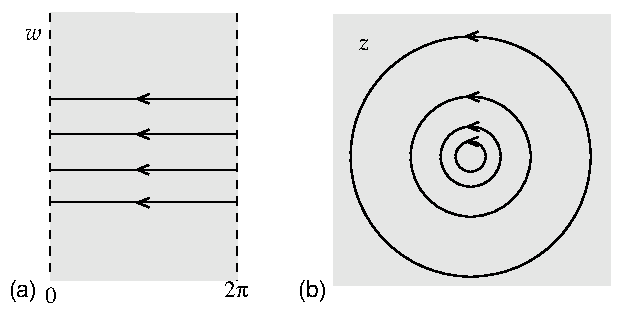
\includegraphics[width=0.8\linewidth]{figures/fig_2_3.pdf}
\caption{閉弦の座標。(a) $w$ 平面の等時刻積分路。破線同士は同一視する。(b) $z$ 平面での同じ積分路。}
\label{fig:2.3}
\end{figure}

正則または反正則な演算子には Laurent 展開が可能である：
\begin{equation}
T_{zz}(z)=\sum_{m=-\infty}^{\infty}\frac{L_m}{z^{m+2}},
\qquad
\widetilde T_{\bar z\bar z}(\bar z)
=\sum_{m=-\infty}^{\infty}\frac{\widetilde L_m}{\bar z^{m+2}}.
\tag{2.6.5}\label{eq:2.6.5}
\end{equation}
Virasoro 生成子として知られる Laurent 係数は、周回積分
\begin{equation}
L_m=\oint_C\frac{dz}{2\pi iz}\,z^{m+2}T_{zz}(z)
\tag{2.6.6}\label{eq:2.6.6}
\end{equation}
で与えられる。ここで $C$ は原点を反時計回りに囲む任意の積分路である。Laurent 展開は、時刻 $\sigma^2=0$ での $w$ 座標系における通常の Fourier 変換と同じである：
\begin{align}
T_{ww}(w)&=-\sum_{m=-\infty}^{\infty}
\exp(im\sigma^1-m\sigma^2)T_m,
\tag{2.6.7a}\label{eq:2.6.7a}\\
T_{\bar w\bar w}(\bar w)&=-\sum_{m=-\infty}^{\infty}
\exp(-im\sigma^1-m\sigma^2)\widetilde T_m,
\tag{2.6.7b}\label{eq:2.6.7b}
\end{align}
ここで
\begin{equation}
T_m=L_m-\delta_{m,0}\frac c{24},\qquad
\widetilde T_m=\widetilde L_m-\delta_{m,0}\frac{\widetilde c}{24}.
\tag{2.6.8}\label{eq:2.6.8}
\end{equation}
$T_0$ の加法的なずれは、テンソル的でない変換 \hyperref[eq:2.4.26]{(2.4.26)}、
\begin{equation}
T_{ww}=(\partial_w z)^2T_{zz}+\frac c{24}
\tag{2.6.9}\label{eq:2.6.9}
\end{equation}
から生じる。$w=\sigma^1+i\sigma^2$ 座標系で時間並進を生成する Hamiltonian $H$ は
\begin{equation}
H=\int_0^{2\pi}\frac{d\sigma^1}{2\pi}\,T_{22}
=L_0+\widetilde L_0-\frac{c+\widetilde c}{24}.
\tag{2.6.10}\label{eq:2.6.10}
\end{equation}
Laurent 展開 \hyperref[eq:2.6.5]{(2.6.5)} にある $+2$ は、$T$ の共形変換により Fourier 展開 \hyperref[eq:2.6.7a]{(2.6.7)} では相殺されていることに注意しよう。同様に、ウェイト $h$ の正則場の Laurent 展開では、指数に $+h$ が含まれる。

時刻 $\operatorname{Im}w=\ln|z|$ が一定の円で経路積分を切り開くと、Virasoro 生成子は通常の意味の演算子になる。（経路積分を切り開くという考え方は付録で展開する。）正則性により、積分 \hyperref[eq:2.6.6]{(2.6.6)} は $C$ に依存せず、とくに時間並進（動径方向のスケール変換）に対して不変である。すなわち、これらは保存電荷であり、共形変換に対応する電荷である。

カレントの OPE が、それに対応する電荷の代数を決めることは重要な事実である。正則カレントの周回積分として与えられる一般の電荷 $Q_i$、$i=1,2$ を考える：
\begin{equation}
Q_i\{C\}=\oint_C\frac{dz}{2\pi i}\,j_i.
\tag{2.6.11}\label{eq:2.6.11}
\end{equation}
組み合わせ
\begin{equation}
Q_1\{C_1\}Q_2\{C_2\}-Q_1\{C_3\}Q_2\{C_2\}
\tag{2.6.12}\label{eq:2.6.12}
\end{equation}
を考え、積分路は図\ref{fig:2.4}(a) に示すものとする。これらは経路積分の積分変数にすぎないので、因子を書いた順序は関係しない（ただし両方の電荷が反交換する場合は別で、その場合には余分な符号が付き、すべての交換子が反交換子になる）。付録で論じるように、経路積分を切り開いて演算子としての解釈を与えるとき、演算子の順序を決めるのは時間の順序であり、ここでは $t_1>t_2>t_3$ である。したがって、組み合わせ \hyperref[eq:2.6.12]{(2.6.12)} を含む経路積分は
\begin{equation}
\widehat Q_1\widehat Q_2-\widehat Q_2\widehat Q_1
\equiv[\widehat Q_1,\widehat Q_2]
\tag{2.6.13}\label{eq:2.6.13}
\end{equation}
の行列要素に対応する。ここで、積分路 $C_2$ 上の一点 $z_2$ を固定すると、積分路 $C_1$ と $C_3$ の差を図\ref{fig:2.4}(b) のように変形できる。したがって交換子は OPE の留数で与えられる：
\begin{equation}
[Q_1,Q_2]\{C_2\}=\oint_{C_2}\frac{dz_2}{2\pi i}\,
\operatorname*{Res}_{z_1\to z_2}j_1(z_1)j_2(z_2).
\tag{2.6.14}\label{eq:2.6.14}
\end{equation}

\begin{figure}[htbp]
\centering
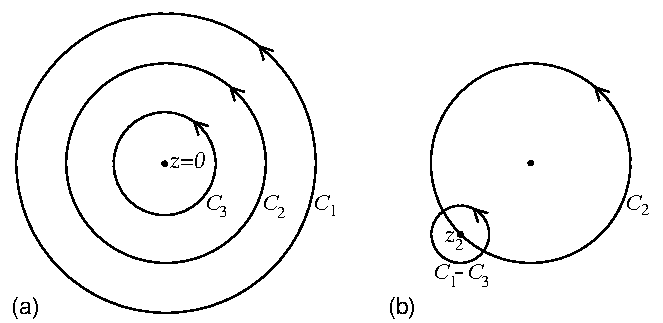
\includegraphics[width=0.8\linewidth]{figures/fig_2_4.pdf}
\caption{(a) $z=0$ を中心とする積分路。(b) 積分路 $C_2$ 上の $z_2$ を固定して、積分路 $C_1-C_3$ を縮める。}
\label{fig:2.4}
\end{figure}

この積分路の議論によって、OPE と交換関係を相互に行き来できる。強調しておくと、保存カレントについて OPE の特異項を知ることは、対応する電荷の交換子代数を知ることと等価である。図\ref{fig:2.4}の計算は、保存電荷 $Q_2\{C_2\}$ を任意の演算子で置き換えた場合にも成り立つ：
\begin{equation}
[Q,\mathcal A(z_2,\bar z_2)]
=\operatorname*{Res}_{z_1\to z_2}j(z_1)\mathcal A(z_2,\bar z_2)
=\frac1{i\epsilon}\delta\mathcal A(z_2,\bar z_2).
\tag{2.6.15}\label{eq:2.6.15}
\end{equation}
これは、電荷 $Q$ が対応する変換 $\delta$ を生成するという、よく知られた主張にほかならない。同様に、反正則カレントの周回積分
\begin{equation}
\widetilde Q\{C\}=-\oint_C\frac{d\bar z}{2\pi i}\,\widetilde j
\tag{2.6.16}\label{eq:2.6.16}
\end{equation}
については、Ward 恒等式と積分路の議論から
\begin{equation}
[\widetilde Q,\mathcal A(z_2,\bar z_2)]
=\operatorname*{Res}_{\bar z_1\to\bar z_2}
\widetilde j(\bar z_1)\mathcal A(z_2,\bar z_2)
=\frac1{i\epsilon}\delta\mathcal A(z_2,\bar z_2)
\tag{2.6.17}\label{eq:2.6.17}
\end{equation}
が従う。

これを Virasoro 生成子 \hyperref[eq:2.6.6]{(2.6.6)} に適用する。この場合、$j_m(z)=z^{m+1}T(z)$ である：
\begin{equation}
\begin{aligned}
&\operatorname*{Res}_{z_1\to z_2}
z_1^{m+1}T(z_1)\,z_2^{n+1}T(z_2)\\
&=\operatorname*{Res}_{z_1\to z_2}z_1^{m+1}z_2^{n+1}
\left(\frac{c}{2z_{12}^4}+\frac2{z_{12}^2}T(z_2)
+\frac1{z_{12}}\partial T(z_2)\right)\\
&=\frac c{12}(\partial^3z_2^{m+1})z_2^{n+1}
+2(\partial z_2^{m+1})z_2^{n+1}T(z_2)
+z_2^{m+n+2}\partial T(z_2)\\
&=\frac c{12}(m^3-m)z_2^{m+n-1}
+(m-n)z_2^{m+n+1}T(z_2)+\text{全微分}.
\end{aligned}
\tag{2.6.18}\label{eq:2.6.18}
\end{equation}
右辺を $z_2$ について周回積分すると、Virasoro 代数
\begin{equation}
[L_m,L_n]=(m-n)L_{m+n}
+\frac c{12}(m^3-m)\delta_{m,-n}
\tag{2.6.19}\label{eq:2.6.19}
\end{equation}
が得られる。$\widetilde L_m$ は中心電荷 $\widetilde c$ を持つ同じ代数を満たす。

したがって、どの CFT にも無限個の保存電荷である Virasoro 生成子が存在し、これらは Hilbert 空間に作用して代数 \hyperref[eq:2.6.19]{(2.6.19)} を満たす。ここではまず、いくつかの簡単な性質に注意しておこう。通常は $L_0$ と $\widetilde L_0$ の固有状態を用いる。生成子 $L_0$ は
\begin{equation}
[L_0,L_n]=-nL_n
\tag{2.6.20}\label{eq:2.6.20}
\end{equation}
を満たす。$\lvert\psi\rangle$ が固有値 $h$ の $L_0$ 固有状態ならば、
\begin{equation}
L_0L_n\lvert\psi\rangle
=L_n(L_0-n)\lvert\psi\rangle
=(h-n)L_n\lvert\psi\rangle,
\tag{2.6.21}\label{eq:2.6.21}
\end{equation}
なので、$L_n\lvert\psi\rangle$ は固有値 $h-n$ の固有状態である。$n<0$ の生成子は $L_0$ 固有値を上げ、$n>0$ の生成子は下げる。

三つの生成子 $L_0$ と $L_{\pm1}$ は、中心電荷を持たない閉じた代数をなす：
\begin{equation}
[L_0,L_1]=-L_1,\qquad
[L_0,L_{-1}]=L_{-1},\qquad
[L_1,L_{-1}]=2L_0.
\tag{2.6.22}\label{eq:2.6.22}
\end{equation}
これは $SL(2,\mathbb R)$ の代数であり、$SU(2)$ とは符号が異なる。ウェイト $(h,0)$ の正則テンソル場 $\mathcal O$ の Laurent 係数、
\begin{equation}
\mathcal O(z)=\sum_{m=-\infty}^{\infty}\frac{\mathcal O_m}{z^{m+h}},
\tag{2.6.23}\label{eq:2.6.23}
\end{equation}
については、OPE \hyperref[eq:2.4.16]{(2.4.16)} から交換関係
\begin{equation}
[L_m,\mathcal O_n]=[(h-1)m-n]\mathcal O_{m+n}
\tag{2.6.24}\label{eq:2.6.24}
\end{equation}
が得られる。ここでも $n>0$ のモードは $L_0$ を下げ、$n<0$ のモードは上げる。

開弦では、
\begin{equation}
0\leq\operatorname{Re}w\leq\pi
\quad\Longleftrightarrow\quad \operatorname{Im}z\geq0
\tag{2.6.25}\label{eq:2.6.25}
\end{equation}
とする。ただし $z=-\exp(-iw)$ である。これらの座標領域を図\ref{fig:2.5}に示す。境界では、エネルギー運動量テンソルは
\begin{equation}
T_{ab}n^at^b=0
\tag{2.6.26}\label{eq:2.6.26}
\end{equation}
を満たす。ここでも $n^a$ と $t^b$ は、それぞれ法線ベクトルと接線ベクトルである。これを見るには、境界が直線になる座標系を考える。境界の存在は法線方向の並進不変性を破るが、接線方向の並進不変性は破らないので、カレント $T_{ab}t^b$ はなお保存される。このとき境界条件 \hyperref[eq:2.6.26]{(2.6.26)} は、このカレントが境界の外へ流れ出す量がゼロであることを述べているにすぎない。今の場合、これは
\begin{equation}
\begin{gathered}
T_{ww}=T_{\bar w\bar w},\quad \operatorname{Re}w=0,\pi
\quad\Longleftrightarrow\quad
T_{zz}=T_{\bar z\bar z},\quad\operatorname{Im}z=0
\end{gathered}
\tag{2.6.27}\label{eq:2.6.27}
\end{equation}
となる。

\begin{figure}[htbp]
\centering
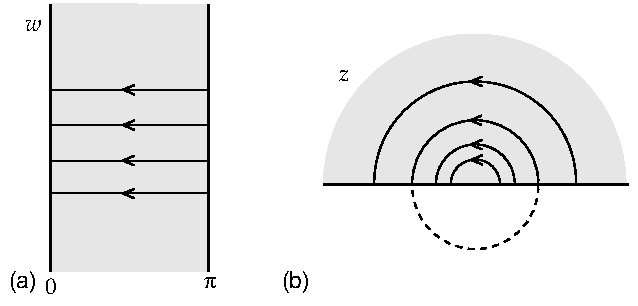
\includegraphics[width=0.8\linewidth]{figures/fig_2_5.pdf}
\caption{開弦の座標。(a) $w$ 平面の等時刻積分路。(b) $z$ 平面での同じ積分路。破線は、二重化の手法で用いる一つの積分路の延長を示す。}
\label{fig:2.5}
\end{figure}

二重化の手法を使うと便利である。$z$ 下半平面での $T_{zz}$ を、$z$ 上半平面にあるその鏡像点 $z'=\bar z$ での $T_{\bar z\bar z}$ の値によって定義する：
\begin{equation}
T_{zz}(z)\equiv T_{\bar z\bar z}(\bar z'),\qquad
\operatorname{Im}z<0.
\tag{2.6.28}\label{eq:2.6.28}
\end{equation}
すると運動方程式と境界条件は、$T_{zz}$ が複素平面全体で正則である、という主張にまとめられる。境界条件が $T$ と $\widetilde T$ を結びつけるので、Virasoro 生成子は一組しかない：
\begin{equation}
\begin{aligned}
L_m&=\frac1{2\pi i}\int_C
\left(dz\,z^{m+1}T_{zz}
-d\bar z\,\bar z^{m+1}T_{\bar z\bar z}\right)\\
&=\frac1{2\pi i}\oint dz\,z^{m+1}T_{zz}(z).
\end{aligned}
\tag{2.6.29}\label{eq:2.6.29}
\end{equation}
第1行の積分路 $C$ は原点を中心とする半円である。第2行では二重化の手法を使い、$L_m$ を閉じた積分路で表した。これらも Virasoro 代数
\begin{equation}
[L_m,L_n]=(m-n)L_{m+n}
+\frac c{12}(m^3-m)\delta_{m,-n}
\tag{2.6.30}\label{eq:2.6.30}
\end{equation}
を満たす。

\subsectionlink{モード展開}
\label{sec:2.7}
\subsubsectionlink*{自由スカラー}

自由場の理論では、場は調和振動子へと分解され、スペクトルとエネルギー運動量テンソルをモードによって表せる。まず閉弦から始める。$X^\mu$ 理論では、$\partial X$ と $\bar\partial X$ はそれぞれ正則および反正則であり、$T$ と同様の Laurent 展開を持つ：
\begin{equation}
\partial X^\mu(z)=-i\left(\frac{\alpha'}2\right)^{1/2}
\sum_{m=-\infty}^{\infty}\frac{\alpha_m^\mu}{z^{m+1}},
\qquad
\bar\partial X^\mu(\bar z)=-i\left(\frac{\alpha'}2\right)^{1/2}
\sum_{m=-\infty}^{\infty}\frac{\widetilde\alpha_m^\mu}{\bar z^{m+1}}.
\tag{2.7.1}\label{eq:2.7.1}
\end{equation}
同値な式として、
\begin{align}
\alpha_m^\mu&=\left(\frac2{\alpha'}\right)^{1/2}
\oint\frac{dz}{2\pi}\,z^m\partial X^\mu(z),
\tag{2.7.2a}\label{eq:2.7.2a}\\
\widetilde\alpha_m^\mu&=-\left(\frac2{\alpha'}\right)^{1/2}
\oint\frac{d\bar z}{2\pi}\,\bar z^m\bar\partial X^\mu(\bar z).
\tag{2.7.2b}\label{eq:2.7.2b}
\end{align}
$X^\mu$ の一価性から $\alpha_0^\mu=\widetilde\alpha_0^\mu$ が従う。さらに、時空並進の Noether カレントは $i\partial_aX^\mu/\alpha'$ なので、時空運動量は
\begin{equation}
p^\mu=\frac1{2\pi i}\oint_C
(dz\,j^\mu-d\bar z\,\widetilde j^\mu)
=\left(\frac2{\alpha'}\right)^{1/2}\alpha_0^\mu
=\left(\frac2{\alpha'}\right)^{1/2}\widetilde\alpha_0^\mu.
\tag{2.7.3}\label{eq:2.7.3}
\end{equation}
展開 \hyperref[eq:2.7.1]{(2.7.1)} を積分すると、
\begin{equation}
X^\mu(z,\bar z)=x^\mu-i\frac{\alpha'}2p^\mu\ln|z|^2
+i\left(\frac{\alpha'}2\right)^{1/2}
\sum_{\substack{m=-\infty\\m\ne0}}^\infty
\frac1m\left(\frac{\alpha_m^\mu}{z^m}
+\frac{\widetilde\alpha_m^\mu}{\bar z^m}\right).
\tag{2.7.4}\label{eq:2.7.4}
\end{equation}

通常の正準交換関係からでも、積分路の議論と $XX$ の OPE からでも、
\begin{align}
[\alpha_m^\mu,\alpha_n^\nu]
&=[\widetilde\alpha_m^\mu,\widetilde\alpha_n^\nu]
=m\delta_{m,-n}\eta^{\mu\nu},
\tag{2.7.5a}\label{eq:2.7.5a}\\
[x^\mu,p^\nu]&=i\eta^{\mu\nu}
\tag{2.7.5b}\label{eq:2.7.5b}
\end{align}
が導かれ、ほかの交換子はゼロとなる。スペクトルは、運動量 $k^\mu$ を持ち、すべての下降モード、すなわち $n>0$ の $\alpha_n^\mu$ によって消滅する状態 $\lvert0;k\rangle$ から始め、上昇モード（$n<0$）を可能なあらゆる仕方で作用させることで与えられる。

次に Virasoro 生成子をモード演算子によって展開したい。$X^\mu$ の Laurent 展開をエネルギー運動量テンソル \hyperref[eq:2.4.4]{(2.4.4)} に代入し、$z$ の同じべきの項を集めると、
\begin{equation}
L_m\sim\frac12\sum_{n=-\infty}^{\infty}
\alpha_{m-n}^\mu\alpha_{\mu n}.
\tag{2.7.6}\label{eq:2.7.6}
\end{equation}
$\sim$ は、演算子の順序を無視したことを示す。$m\ne0$ の場合、展開 \hyperref[eq:2.7.6]{(2.7.6)} はそのままで明確に定義され、正しい。各項のモード演算子同士は交換するので、順序は問題にならない。$m=0$ では、下降演算子を右に置き、正規順序定数を導入する：
\begin{equation}
L_0=\frac{\alpha'p^2}{4}
+\sum_{n=1}^\infty(\alpha_{-n}^\mu\alpha_{\mu n})+a^X.
\tag{2.7.7}\label{eq:2.7.7}
\end{equation}
第1.3節でも同じ問題に出会い、そのときは発見的な方法で扱った。今は、左辺には $:\ :$ 順序にしたエネルギー運動量テンソルの Laurent 係数という有限で曖昧さのない定義があるので、正規順序定数も有限で計算可能である。決め方はいくつかある。最も簡単なのは Virasoro 代数を用いるもので、
\begin{equation}
2L_0\lvert0;0\rangle
=(L_1L_{-1}-L_{-1}L_1)\lvert0;0\rangle=0,
\tag{2.7.8}\label{eq:2.7.8}
\end{equation}
したがって
\begin{equation}
a^X=0.
\tag{2.7.9}\label{eq:2.7.9}
\end{equation}
ここでは、既知の $L_1$ と $L_{-1}$ の形を用いた。それぞれの各項は、下降演算子か $p^\mu$ のどちらかを含むので、$\lvert0;0\rangle$ を消滅させる。

Virasoro 代数の中心電荷は OPE から決めた。モード演算子で表した Virasoro 生成子の式から直接決めることもできるが、少し注意が必要である。これは演習2.11とする。

新しい記法を導入しよう。記号 $\canorm{\phantom X}$ は生成・消滅演算子の正規順序を表し、すべての下降演算子をすべての上昇演算子の右に置き、反交換する演算子を入れ替えるたびに負号を付ける。この定義では、$p^\mu$ は下降演算子に、$x^\mu$ は上昇演算子に含める。この記法なら、$a^X=0$ なので
\begin{equation}
L_m=\frac12\sum_{n=-\infty}^{\infty}
\canorm{\alpha_{m-n}^\mu\alpha_{\mu n}}
\tag{2.7.10}\label{eq:2.7.10}
\end{equation}
と書ける。

これで二種類の正規順序を導入した。共形正規順序 $:\ :$（単に「正規順序」と呼ぶときはこれを意味する）と、生成・消滅演算子の正規順序 $\canorm{\phantom X}$ である。前者は、OPE と共形変換性が簡単な演算子を与える点で便利である。読者にはおそらく後者の方がなじみ深いだろうが、こちらは演算子の行列要素を求めるのに便利である。この二つの関係を求めよう。まず時間順序積と生成・消滅演算子の正規順序積を比較する。$|z|>|z'|$ を満たす積 $X^\mu(z,\bar z)X^\nu(z',\bar z')$ にモード展開を代入し、$X^\mu(z,\bar z)$ に含まれる下降演算子を右へ動かす。交換子を追跡すると、
\begin{equation}
\begin{aligned}
X^\mu(z,\bar z)X^\nu(z',\bar z')
&=\canorm{X^\mu(z,\bar z)X^\nu(z',\bar z')}\\
&\quad+\frac{\alpha'}2\eta^{\mu\nu}
\left[-\ln|z|^2+\sum_{m=1}^{\infty}\frac1m
\left(\frac{z'^m}{z^m}+\frac{\bar z'^m}{\bar z^m}\right)\right]\\
&=\canorm{X^\mu(z,\bar z)X^\nu(z',\bar z')}
-\frac{\alpha'}2\eta^{\mu\nu}\ln|z-z'|^2.
\end{aligned}
\tag{2.7.11}\label{eq:2.7.11}
\end{equation}
$|z|>|z'|$ なので、ここで左辺は時間順序積であり、和は収束する。定義 \hyperref[eq:2.1.21a]{(2.1.21)} は、時間順序積と共形正規順序積の関係を与えていた（式 \hyperref[eq:2.1.21a]{(2.1.21)} は経路積分の言葉で書かれていたので、その右辺の積は演算子形式では時間順序積になる）。それは関係 \hyperref[eq:2.7.11]{(2.7.11)} と同じなので、
\begin{equation}
\canorm{X^\mu(z,\bar z)X^\nu(z',\bar z')}
=:X^\mu(z,\bar z)X^\nu(z',\bar z'):.
\tag{2.7.12}\label{eq:2.7.12}
\end{equation}
このような関係は一般の CFT では成立しない。実際、$p^\mu$ を下降演算子と一緒に分類した多少恣意的な選択は、この簡単な結果を得ることも目的の一つであった。また、たとえば $z$ ではなく $w$ について共形正規順序にした演算子でも、この関係は成立しない。式 \hyperref[eq:2.7.12]{(2.7.12)} からモード展開 \hyperref[eq:2.7.10]{(2.7.10)} を直ちに書け、$a^X=0$ の二つ目の導出が得られる。

三つ以上の $X^\mu$ の生成・消滅演算子の正規順序積は、$:\ :$ 順序と同じ組み合わせ論的性質を持つ。すなわち、すべての差し引きについて和を取ることで時間順序積から得られる。これは場の理論の Wick の定理である。また、ある正規順序で定義した演算子を別の正規順序へ変換するには、2点関数の差を用いてすべての差し引きについて和を取ればよい。すなわち、二種類の順序が
\begin{equation}
[X^\mu(z,\bar z)X^\nu(z',\bar z')]_1
=[X^\mu(z,\bar z)X^\nu(z',\bar z')]_2
+\eta^{\mu\nu}\Delta(z,\bar z,z',\bar z')
\tag{2.7.13}\label{eq:2.7.13}
\end{equation}
を満たすならば、一般の演算子 $\mathcal F$ について
\begin{equation}
[\mathcal F]_1=
\exp\left(\frac12\int d^2z\,d^2z'\,
\Delta(z,\bar z,z',\bar z')
\frac{\delta}{\delta X^\mu(z,\bar z)}
\frac{\delta}{\delta X_\mu(z',\bar z')}\right)[\mathcal F]_2.
\tag{2.7.14}\label{eq:2.7.14}
\end{equation}

線形ディラトン CFT では、Laurent 展開と交換関係は変わらないが、Virasoro 生成子に追加項が含まれる：
\begin{equation}
L_m=\frac12\sum_{n=-\infty}^\infty
\canorm{\alpha_{m-n}^\mu\alpha_{\mu n}}
+i\left(\frac{\alpha'}2\right)^{1/2}(m+1)V^\mu\alpha_{\mu m}.
\tag{2.7.15}\label{eq:2.7.15}
\end{equation}

\subsubsectionlink*{\texorpdfstring{$bc$}{bc} CFT}

場 $b$ と $c$ は Laurent 展開
\begin{equation}
b(z)=\sum_{m=-\infty}^\infty\frac{b_m}{z^{m+\lambda}},
\qquad
c(z)=\sum_{m=-\infty}^\infty\frac{c_m}{z^{m+1-\lambda}}
\tag{2.7.16}\label{eq:2.7.16}
\end{equation}
を持つ。厳密には、これらが Laurent 展開となるのは $\lambda$ が整数の場合だけであり、ここではそう仮定する。半整数の場合も興味深いが、第10章で詳しく扱う。OPE から反交換関係
\begin{equation}
\{b_m,c_n\}=\delta_{m,-n}
\tag{2.7.17}\label{eq:2.7.17}
\end{equation}
が得られる。まず、すべての $n>0$ の演算子によって消滅する状態を考える。$b_0,c_0$ の振動子代数は、そのような基底状態を二つ、$\lvert\downarrow\rangle$ と $\lvert\uparrow\rangle$、生成する。これらの性質は
\begin{align}
b_0\lvert\downarrow\rangle&=0,\qquad
b_0\lvert\uparrow\rangle=\lvert\downarrow\rangle,
\tag{2.7.18a}\label{eq:2.7.18a}\\
c_0\lvert\downarrow\rangle&=\lvert\uparrow\rangle,\qquad
c_0\lvert\uparrow\rangle=0,
\tag{2.7.18b}\label{eq:2.7.18b}\\
b_n\lvert\downarrow\rangle&=b_n\lvert\uparrow\rangle
=c_n\lvert\downarrow\rangle=c_n\lvert\uparrow\rangle=0,\qquad n>0.
\tag{2.7.18c}\label{eq:2.7.18c}
\end{align}
一般の状態は、これらの状態に $n<0$ のモードを各々高々一度ずつ作用させて得られる（これらは反交換するためである）。後に明らかになる理由により、$b_0$ を下降演算子に、$c_0$ を上昇演算子に分類するのが慣例なので、$\lvert\downarrow\rangle$ をゴースト真空 $\lvert0\rangle$ として特別に選ぶ。弦理論では、どちらも $\lambda=2$ の正則な $bc$ 理論と反正則な $\widetilde b\widetilde c$ 理論を持つ。したがって閉弦のスペクトルには、上の系を二つ複製したものの積が含まれる。

Virasoro 生成子は
\begin{equation}
L_m=\sum_{n=-\infty}^\infty(m\lambda-n)
\canorm{b_nc_{m-n}}+\delta_{m,0}a^{\mathrm g}.
\tag{2.7.19}\label{eq:2.7.19}
\end{equation}
順序定数は式 \hyperref[eq:2.7.8]{(2.7.8)} と同じように決められ、
\begin{equation}
\begin{aligned}
2L_0\lvert\downarrow\rangle
&=(L_1L_{-1}-L_{-1}L_1)\lvert\downarrow\rangle\\
&=(\lambda b_0c_1)[(1-\lambda)b_{-1}c_0]\lvert\downarrow\rangle
=\lambda(1-\lambda)\lvert\downarrow\rangle.
\end{aligned}
\tag{2.7.20}\label{eq:2.7.20}
\end{equation}
したがって $a^{\mathrm g}=\frac12\lambda(1-\lambda)$ であり、
\begin{equation}
L_m=\sum_{n=-\infty}^\infty(m\lambda-n)
\canorm{b_nc_{m-n}}+\frac{\lambda(1-\lambda)}2\delta_{m,0}.
\tag{2.7.21}\label{eq:2.7.21}
\end{equation}
この定数は、この CFT における $:\ :$ と $\canorm{\phantom X}$ の関係を求めることでも得られる（演習2.13、2.14）。

ゴースト数カレント \hyperref[eq:2.5.14]{(2.5.14)}、$j=-:bc:$ の電荷は
\begin{equation}
\begin{aligned}
N^{\mathrm g}&=-\frac1{2\pi i}\int_0^{2\pi}dw\,j_w\\
&=\sum_{n=1}^\infty(c_{-n}b_n-b_{-n}c_n)+c_0b_0-\frac12.
\end{aligned}
\tag{2.7.22}\label{eq:2.7.22}
\end{equation}
これは
\begin{equation}
[N^{\mathrm g},b_m]=-b_m,\qquad
[N^{\mathrm g},c_m]=c_m
\tag{2.7.23}\label{eq:2.7.23}
\end{equation}
を満たすので、$c$ の励起数から $b$ の励起数を引いたものを数える。基底状態のゴースト数は $\pm\frac12$ である：
\begin{equation}
N^{\mathrm g}\lvert\downarrow\rangle=-\frac12\lvert\downarrow\rangle,
\qquad
N^{\mathrm g}\lvert\uparrow\rangle=\frac12\lvert\uparrow\rangle.
\tag{2.7.24}\label{eq:2.7.24}
\end{equation}
これは演習2.13で求める順序定数の値に依存するが、基底状態の平均ゴースト数はゼロになるべきだという理由から推測することもできる。ゴースト数は $b\leftrightarrow c$ の下で符号を変えるからである。

$\beta\gamma$ 理論も同様である。詳細は、それが必要になる第10章まで先送りする。

\subsubsectionlink*{開弦}

開弦では、Neumann 境界条件は実軸上で $\partial_zX^\mu=\partial_{\bar z}X^\mu$ となる。境界条件は展開 \hyperref[eq:2.7.1]{(2.7.1)} で $\alpha_m^\mu=\widetilde\alpha_m^\mu$ を要求するので、モードは一組しかない。時空運動量の積分 \hyperref[eq:2.7.3]{(2.7.3)} は半円上だけを走るため、規格化は今度は
\begin{equation}
\alpha_0^\mu=(2\alpha')^{1/2}p^\mu.
\tag{2.7.25}\label{eq:2.7.25}
\end{equation}
したがって $X^\mu$ の展開は
\begin{equation}
X^\mu(z,\bar z)=x^\mu-i\alpha'p^\mu\ln|z|^2
+i\left(\frac{\alpha'}2\right)^{1/2}
\sum_{\substack{m=-\infty\\m\ne0}}^\infty
\frac{\alpha_m^\mu}{m}(z^{-m}+\bar z^{-m}).
\tag{2.7.26}\label{eq:2.7.26}
\end{equation}
また、
\begin{equation}
L_0=\alpha'p^2+\sum_{n=1}^\infty\alpha_{-n}^\mu\alpha_{\mu n}.
\tag{2.7.27}\label{eq:2.7.27}
\end{equation}
交換関係は以前と同じである：
\begin{equation}
[\alpha_m^\mu,\alpha_n^\nu]=m\delta_{m,-n}\eta^{\mu\nu},
\qquad [x^\mu,p^\nu]=i\eta^{\mu\nu}.
\tag{2.7.28}\label{eq:2.7.28}
\end{equation}

$bc$ 理論では、弦に関係する境界条件は、境界が実軸となる $z$ 座標を用いて
\begin{equation}
c(z)=\widetilde c(\bar z),\qquad
b(z)=\widetilde b(\bar z),\qquad\operatorname{Im}z=0
\tag{2.7.29}\label{eq:2.7.29}
\end{equation}
と書かれる。すると二重化の手法によって、上半平面の正則場と反正則場を、全平面の正則場として表せる：
\begin{equation}
c(z)\equiv\widetilde c(\bar z'),\qquad
b(z)\equiv\widetilde b(\bar z'),\qquad
\operatorname{Im}z\leq0,\quad z'=\bar z.
\tag{2.7.30}\label{eq:2.7.30}
\end{equation}
したがって開弦は、$b$ と $c$ について、それぞれ一組の Laurent モードを持つ。

\subsectionlink{頂点演算子}
\label{sec:2.8}

場の量子論には、一方で理論の状態空間があり、他方で局所演算子の集合がある。共形場理論では、CFT を円上で量子化すると、これらの間に簡単で有用な同型対応がある。$w$ 座標で半無限円筒
\begin{equation}
0\leq\operatorname{Re}w\leq2\pi,\qquad
w\sim w+2\pi,\qquad \operatorname{Im}w\leq0
\tag{2.8.1}\label{eq:2.8.1}
\end{equation}
を考える。これは座標 $z=\exp(-iw)$ では単位円板に写る。その様子を図\ref{fig:2.6}に示す。$w$ 座標で経路積分を定義するには、とくに $\operatorname{Im}w\to-\infty$ での境界条件を指定しなければならない。すなわち、初期状態を指定する必要がある。$z$ 座標では $\operatorname{Im}w=-\infty$ は原点に写るので、これはその点での場の振る舞いを指定することと同じである。実質的には、これにより原点に局所演算子を定義しており、その状態に対応する頂点演算子と呼ばれる。逆向きに進むと、原点に演算子 $\mathcal A$ を置いた円板上の経路積分は、初期状態 $\lvert\mathcal A\rangle$ を指定した円筒上の経路積分に写る。

自由場の理論では、この同型対応の具体的な形を容易に求められる。図\ref{fig:2.6}(a) のように、保存電荷 $Q$ が状態 $\lvert\mathcal A\rangle$ に作用しているとする。図\ref{fig:2.6}(b) の周回積分を OPE で評価すれば、対応する局所演算子を求められる。これを使い、単位演算子に対応する状態 $\lvert1\rangle$ を同定しよう。原点に演算子がなければ、$\partial X^\mu$ と $\bar\partial X^\mu$ は図\ref{fig:2.6}(b) の $Q$ の積分路の内部で、それぞれ正則および反正則である。したがって、$m\geq0$ の $\alpha_m^\mu$ と $\widetilde\alpha_m^\mu$ を定義する周回積分 \hyperref[eq:2.7.2a]{(2.7.2)} には極がなく、ゼロになる。つまり、$\lvert1\rangle$ はこれらのモードによって消滅する。これにより、この状態が基底状態であると分かる：
\begin{equation}
\lvert1\rangle=\lvert0;0\rangle.
\tag{2.8.2}\label{eq:2.8.2}
\end{equation}
規格化は便宜上このように選んだ。

\begin{figure}[htbp]
\centering
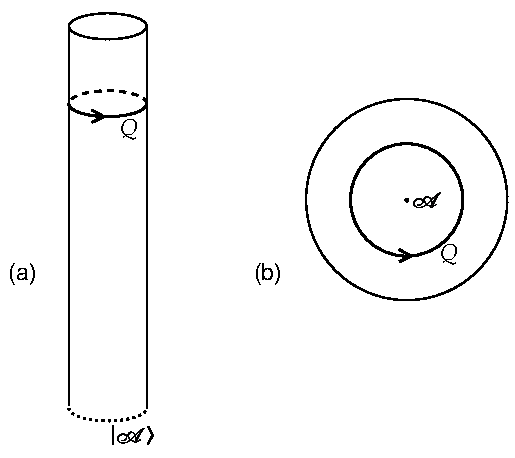
\includegraphics[width=0.8\linewidth]{figures/fig_2_6.pdf}
\caption{(a) 初期状態 $\lvert\mathcal A\rangle$ と電荷 $Q$ を持つ、$w$ での半無限円筒。(b) それと共形的に等価な単位円板。局所演算子 $\mathcal A$ と、$Q$ の周回積分を示す。}
\label{fig:2.6}
\end{figure}

次に、たとえば $m$ が正の状態 $\alpha_{-m}^\mu\lvert1\rangle$ を考える。図\ref{fig:2.6}(b) に移り、$Q=\alpha_{-m}^\mu$ が単位演算子を囲むようにすると、場は積分路の内部で正則なので、$m\geq1$ について
\begin{equation}
\alpha_{-m}^\mu=
\left(\frac2{\alpha'}\right)^{1/2}
\oint\frac{dz}{2\pi}\,z^{-m}\partial X^\mu(z)
\ \longrightarrow\
\left(\frac2{\alpha'}\right)^{1/2}
\frac{i}{(m-1)!}\partial^m X^\mu(0)
\tag{2.8.3}\label{eq:2.8.3}
\end{equation}
と評価できる。したがって、
\begin{equation}
\alpha_{-m}^\mu\lvert1\rangle\cong
\left(\frac2{\alpha'}\right)^{1/2}
\frac{i}{(m-1)!}\partial^m X^\mu(0),\qquad m\geq1.
\tag{2.8.4}\label{eq:2.8.4}
\end{equation}
同様に、
\begin{equation}
\widetilde\alpha_{-m}^\mu\lvert1\rangle\cong
\left(\frac2{\alpha'}\right)^{1/2}
\frac{i}{(m-1)!}\bar\partial^m X^\mu(0),\qquad m\geq1.
\tag{2.8.5}\label{eq:2.8.5}
\end{equation}

この対応は、$\alpha_{-m}^\mu$ または $\widetilde\alpha_{-m}^\mu$ が一般の状態 $\lvert\mathcal A\rangle$ に作用する場合にも成立する。$: \mathcal A(0,0):$ を任意の正規順序演算子とすると、$\partial X^\mu(z)$ と $:\mathcal A(0,0):$ の演算子積には特異性があり得るが、$m>0$ について
\begin{equation}
\alpha_{-m}^\mu:\mathcal A(0,0):
=:\alpha_{-m}^\mu\mathcal A(0,0):
\tag{2.8.6}\label{eq:2.8.6}
\end{equation}
を確かめるのは難しくない。縮約の周回積分には決して1位の極が現れないからである。したがって、同じ操作 \hyperref[eq:2.8.3]{(2.8.3)} を正規順序の内部で行え、複数の $\alpha$ 振動子を励起した状態は、対応する演算子の $:\ :$ 正規順序積となる：
\begin{align}
\alpha_{-m}^\mu&\longrightarrow
i\left(\frac2{\alpha'}\right)^{1/2}
\frac1{(m-1)!}\partial^mX^\mu(0),\qquad m\geq1,
\tag{2.8.7a}\label{eq:2.8.7a}\\
\widetilde\alpha_{-m}^\mu&\longrightarrow
i\left(\frac2{\alpha'}\right)^{1/2}
\frac1{(m-1)!}\bar\partial^mX^\mu(0),\qquad m\geq1.
\tag{2.8.7b}\label{eq:2.8.7b}
\end{align}
同様に、
\begin{equation}
x_0^\mu\longrightarrow X^\mu(0,0).
\tag{2.8.8}\label{eq:2.8.8}
\end{equation}
どの状態も、式 \hyperref[eq:2.8.7a]{(2.8.7)} と \hyperref[eq:2.8.8]{(2.8.8)} の左辺の演算子を $\lvert1\rangle$ に作用させて得られる。すると、この状態に対応する演算子は、右辺の対応する局所演算子の $:\ :$ 正規順序積で与えられる。たとえば、
\begin{equation}
\lvert0;k\rangle\cong:e^{ik\cdot X(0,0)}:.
\tag{2.8.9}\label{eq:2.8.9}
\end{equation}
これは容易に理解できる。並進 $X^\mu\to X^\mu+a^\mu$ の下で、状態と対応する演算子はどちらも $\exp(ik\cdot a)$ を掛けるという同じ変換を受けるからである。

同じ方法は $bc$ 理論にも適用できる。明確さのため、ボース弦理論で関心のある $\lambda=2$ の場合に限定し、一般化は読者に任せる。Laurent 展開 \hyperref[eq:2.7.16]{(2.7.16)} と積分路の議論から、
\begin{equation}
b_m\lvert1\rangle=0,\quad m\geq-1,\qquad
c_m\lvert1\rangle=0,\quad m\geq2
\tag{2.8.10}\label{eq:2.8.10}
\end{equation}
が従う。$b$ と $c$ の共形ウェイトにより Laurent 展開の指数がずれるため、単位演算子はもはや基底状態へは写らないことに注意しよう。代わりに、関係 \hyperref[eq:2.8.10]{(2.8.10)} から
\begin{equation}
\lvert1\rangle=b_{-1}\lvert\downarrow\rangle
\tag{2.8.11}\label{eq:2.8.11}
\end{equation}
と決まる。上昇演算子の対応を求めるのは容易で、
\begin{align}
b_{-m}&\longrightarrow\frac1{(m-2)!}\partial^{m-2}b(0),
\qquad m\geq2,
\tag{2.8.12a}\label{eq:2.8.12a}\\
c_{-m}&\longrightarrow\frac1{(m+1)!}\partial^{m+1}c(0),
\qquad m\geq-1.
\tag{2.8.12b}\label{eq:2.8.12b}
\end{align}

ゴースト数 $-\frac32$ の状態 $b_{-1}\lvert\downarrow\rangle$ がゴースト数0の単位演算子に写り、ゴースト数 $-\frac12$ の状態 $\lvert\downarrow\rangle$ がゴースト数1の演算子 $c$ に写ることに注意しよう。この差は、ゴースト数カレントのテンソル的でない性質 \hyperref[eq:2.5.17]{(2.5.17)}、
\begin{equation}
(\partial_z w)j_w(w)=j_z(z)
+q_0\frac{\partial_z^2w}{\partial_z w}
=j_z(z)-\frac{q_0}{z}
\tag{2.8.13}\label{eq:2.8.13}
\end{equation}
から生じる。ここで $q_0=\lambda-\frac12=\frac32$ である。状態のゴースト数は慣例として円筒座標系の式 $N^{\mathrm g}$、式 \hyperref[eq:2.7.22]{(2.7.22)}、で定義する。一方、図\ref{fig:2.6}の積分路の議論が頂点演算子のゴースト数に結びつけるのは、動径座標系の電荷
\begin{equation}
Q^{\mathrm g}\equiv\frac1{2\pi i}\oint dz\,j_z
=N^{\mathrm g}+q_0
\tag{2.8.14}\label{eq:2.8.14}
\end{equation}
である。これはほかの電荷にも当てはまる。テンソルカレントなら、状態と対応する演算子の電荷は等しい。

以上の大部分は $\beta\gamma$ 理論にも拡張できるが、超弦にはいくつかの複雑な点があるので、第10章まで先送りする。

この節の考え方はすべて開弦にも拡張できる。半無限帯
\begin{equation}
0\leq\operatorname{Re}w\leq\pi,\qquad \operatorname{Im}w\leq0
\tag{2.8.15}\label{eq:2.8.15}
\end{equation}
は $z=-\exp(-iw)$ によって、上半平面と単位円の内部の共通部分である半円板に写る。初期状態はここでも原点に写るが、原点は境界上にあるため、同型対応
\begin{equation}
\text{境界上の局所演算子}
\quad\longleftrightarrow\quad
\text{区間上の状態}
\tag{2.8.16}\label{eq:2.8.16}
\end{equation}
がある。上の議論と並行する詳細は読者に任せる。ここでも、場を正則性によって下半平面へ拡張する二重化の手法が、積分路の議論を行うのに便利である。

\subsubsectionlink*{経路積分による導出}

状態と演算子の同型対応は重要だがなじみの薄い考え方なので、より明示的な経路積分による導出も与えておくと有用である。$z$ 平面の単位円板を考え、原点に局所演算子 $\mathcal A$ を置き、経路積分の場 $\phi$ を単位円上である特定の境界値 $\phi_{\mathrm b}$ に固定する。$\phi_{\mathrm b}$ を固定したまま、円板の内部の場 $\phi_{\mathrm i}$ について経路積分すると、ある汎関数 $\Psi_{\mathcal A}[\phi_{\mathrm b}]$ が得られる：
\begin{equation}
\Psi_{\mathcal A}[\phi_{\mathrm b}]
=\int[d\phi_{\mathrm i}]_{\phi_{\mathrm b}}\,
\exp(-S[\phi_{\mathrm i}])\mathcal A(0).
\tag{2.8.17}\label{eq:2.8.17}
\end{equation}
場の汎関数は状態の Schrödinger 表現なので、これは演算子から状態への写像である。各場の配位に複素振幅を割り当てる Schrödinger 表現には、多くの用途がある。場の理論の教科書ではしばしば Fock 空間表示に重点が置かれ、Schrödinger 表現は省かれる。

逆向きに進むには、ある状態 $\Psi[\phi_{\mathrm b}]$ から始める。外側の円上の場 $\phi_{\mathrm b}$ を固定し、内側の円上の場 $\phi'_{\mathrm b}$ を次のように積分する、環状領域 $1\geq|z|\geq r$ 上の経路積分を考える：
\begin{equation}
\int[d\phi'_{\mathrm b}]
[d\phi_{\mathrm i}]_{\phi_{\mathrm b},\phi'_{\mathrm b}}
\exp(-S[\phi_{\mathrm i}])\,
r^{-L_0-\widetilde L_0}\Psi[\phi'_{\mathrm b}].
\tag{2.8.18}\label{eq:2.8.18}
\end{equation}
すなわち、積分は状態（汎関数）$r^{-L_0-\widetilde L_0}\Psi[\phi'_{\mathrm b}]$ によって重み付けされる。さて、環状領域上の経路積分は、$|z|=r$ から $|z|=1$ への伝播にほかならず、演算子 $r^{+L_0+\widetilde L_0}$ の作用と同じである。これが $\Psi$ に作用している演算子を打ち消すので、経路積分 \hyperref[eq:2.8.18]{(2.8.18)} は再び $\Psi[\phi_{\mathrm b}]$ となる。ここで $r\to0$ の極限を取る。環状領域は円板となり、内側の円上の経路積分の極限は、原点にある局所演算子を定義すると考えられる。構成の仕方から、この演算子を挿入した円板上の経路積分は、境界に $\Psi[\phi_{\mathrm b}]$ を再現する。

一つの自由スカラー場 $X$ について、これを具体的に計算しよう。単位円上で
\begin{equation}
X_{\mathrm b}(\theta)=\sum_{n=-\infty}^\infty X_ne^{in\theta},
\qquad X_n^*=X_{-n}
\tag{2.8.19}\label{eq:2.8.19}
\end{equation}
と展開する。したがって、境界状態 $\Psi[X_{\mathrm b}]$ は、すべての $X_n$ の関数とみなせる。まず、挿入のない経路積分
\begin{equation}
\Psi_1[X_{\mathrm b}]
=\int[dX_{\mathrm i}]_{X_{\mathrm b}}\,
\exp\left(-\frac1{2\pi\alpha'}
\int d^2z\,\partial X\bar\partial X\right)
\tag{2.8.20}\label{eq:2.8.20}
\end{equation}
によって与えられる、単位演算子に対応する状態を同定しよう。これを通常の Gauss 積分の方法で評価する。$X_{\mathrm i}$ を古典的な部分とゆらぎに分ける：
\begin{align}
X_{\mathrm i}&=X_{\mathrm{cl}}+X'_{\mathrm i},
\tag{2.8.21a}\label{eq:2.8.21a}\\
X_{\mathrm{cl}}(z,\bar z)
&=X_0+\sum_{n=1}^\infty(z^nX_n+\bar z^nX_{-n}).
\tag{2.8.21b}\label{eq:2.8.21b}
\end{align}
この定義によって、$X_{\mathrm{cl}}$ は運動方程式を満たし、$X'_{\mathrm i}$ は境界でゼロになる。すると経路積分は分離され、
\begin{equation}
\Psi_1[X_{\mathrm b}]=\exp(-S_{\mathrm{cl}})
\int[dX'_{\mathrm i}]_{X_{\mathrm b}=0}\,
\exp\left(-\frac1{2\pi\alpha'}
\int d^2z\,\partial X'\bar\partial X'\right),
\tag{2.8.22}\label{eq:2.8.22}
\end{equation}
ここで
\begin{equation}
\begin{aligned}
S_{\mathrm{cl}}&=\frac1{2\pi\alpha'}
\sum_{m,n=1}^\infty mnX_mX_{-n}
\int_{|z|<1}d^2z\,z^{m-1}\bar z^{n-1}\\
&=\frac1{\alpha'}\sum_{m=1}^\infty mX_mX_{-m}.
\end{aligned}
\tag{2.8.23}\label{eq:2.8.23}
\end{equation}
$X'_{\mathrm i}$ の積分は境界条件に依存しない定数なので、
\begin{equation}
\Psi_1[X_{\mathrm b}]\propto
\exp\left(-\frac1{\alpha'}\sum_{m=1}^\infty mX_mX_{-m}\right).
\tag{2.8.24}\label{eq:2.8.24}
\end{equation}
これは Gauss 関数であり、実際に基底状態である。このことを見るため、上昇演算子と下降演算子を Schrödinger 基底で書く：
\begin{align}
\alpha_n&=-\frac{in}{(2\alpha')^{1/2}}X_{-n}
-i\left(\frac{\alpha'}2\right)^{1/2}\frac{\partial}{\partial X_n},
\tag{2.8.25a}\label{eq:2.8.25a}\\
\widetilde\alpha_n&=-\frac{in}{(2\alpha')^{1/2}}X_n
-i\left(\frac{\alpha'}2\right)^{1/2}\frac{\partial}{\partial X_{-n}}.
\tag{2.8.25b}\label{eq:2.8.25b}
\end{align}
これは $|z|=1$ での Laurent 展開とモード代数から従う。\hyperref[eq:2.8.24]{(2.8.24)} に作用させると、
\begin{equation}
\alpha_n\Psi_1[X_{\mathrm b}]
=\widetilde\alpha_n\Psi_1[X_{\mathrm b}]=0,\qquad n\geq0
\tag{2.8.26}\label{eq:2.8.26}
\end{equation}
となるので、これは確かに基底状態である。したがって、
\begin{equation}
\lvert1\rangle\propto\lvert0;0\rangle.
\tag{2.8.27}\label{eq:2.8.27}
\end{equation}
ここで経路積分全体の規格化を追跡しようとする代わりに、$\lvert1\rangle=\lvert0;0\rangle$ と定義する。

もう一つ容易に計算できるのは、$\partial^kX$ に対応する状態である。これは結果に $\partial^kX_{\mathrm{cl}}(0)=k!X_k$ という因子を付け加えるだけなので、
\begin{equation}
\lvert\partial^kX\rangle=k!X_k\Psi_1
=-i\left(\frac{\alpha'}2\right)^{1/2}
(k-1)!\alpha_{-k}\lvert0;0\rangle,
\tag{2.8.28}\label{eq:2.8.28}
\end{equation}
となり、$\bar\partial^kX$ についても同様である。これは $X$ の指数関数と微分のあらゆる積へ拡張できる。共形正規順序は、ちょうど $X'_{\mathrm i}$ の経路積分の効果を打ち消す。

\subsectionlink{状態と演算子についてさらに}
\label{sec:2.9}
\subsubsectionlink*{OPE}

この節では、状態と演算子の対応をさらに応用する。最初は、図\ref{fig:2.7}に示す OPE の簡単で一般的な導出である。$|z|<1$ として、積
\begin{equation}
\mathcal A_i(z,\bar z)\mathcal A_j(0,0)
\tag{2.9.1}\label{eq:2.9.1}
\end{equation}
を考える。経路積分を、単位円板の内部の場 $\phi_{\mathrm i}$ の積分、単位円上の場 $\phi_{\mathrm b}$ の積分、および単位円板の外部の場 $\phi_{\mathrm e}$ の積分に分けられる。このように経路積分を切り開くことは付録で詳しく論じる。前節の最後の議論と同様に、$\phi_{\mathrm i}$ の積分の後には $\phi_{\mathrm b}$ のある汎関数が残る。それを $\Psi_{ij,z,\bar z}[\phi_{\mathrm b}]$ と呼ぼう。状態と演算子の対応によれば、これは適切な局所演算子 $\mathcal A_{ij,z,\bar z}(0,0)$ を入れた円板を貼り戻すことと等価であり、これで導出は終わりである。標準的な形にするため、$L_0,\widetilde L_0$ の固有状態の完全系で展開する：
\begin{equation}
\mathcal A_{ij,z,\bar z}
=\sum_k z^{h_k-h_i-h_j}
\bar z^{\widetilde h_k-\widetilde h_i-\widetilde h_j}
c^k_{ij}\mathcal A_k.
\tag{2.9.2}\label{eq:2.9.2}
\end{equation}
$z$ と $\bar z$ への依存性は、式 \hyperref[eq:2.4.20]{(2.4.20)} と同じく共形ウェイトによって決まる。OPE の収束は、量子力学における完全系の通常の収束にほかならない。この構成は、$|z'|\leq|z|$ を満たすほかの演算子が存在せず、半径 $|z|+\epsilon$ の円で切れる限り可能である。

\begin{figure}[htbp]
\centering
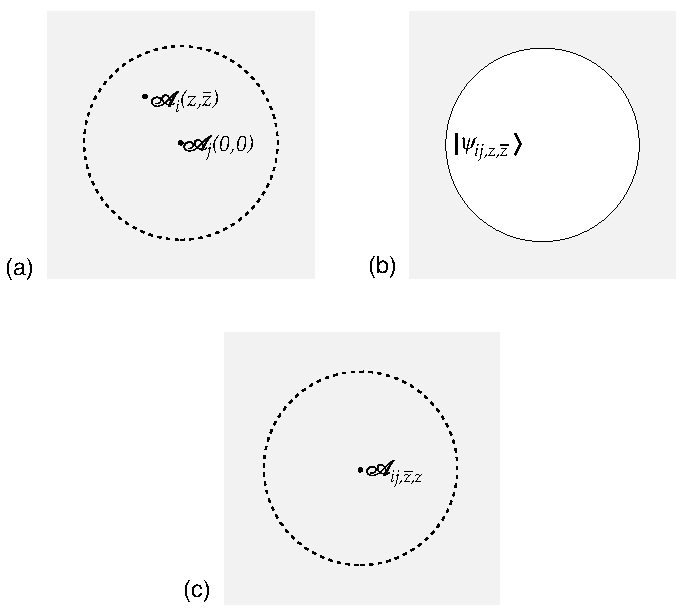
\includegraphics[width=0.8\linewidth]{figures/fig_2_7.pdf}
\caption{(a) 二つの局所演算子を持つ世界面。(b) 円板の内部の場を積分すると、境界状態 $\lvert\psi_{ij,z,\bar z}\rangle$ が得られる。(c) 対応する局所演算子を持つ円板を縫い合わせる。確定したウェイトを持つ演算子で展開すると OPE が得られる。}
\label{fig:2.7}
\end{figure}

三つの演算子
\begin{equation}
\mathcal A_i(0,0)\mathcal A_j(1,1)\mathcal A_k(z,\bar z)
\tag{2.9.3}\label{eq:2.9.3}
\end{equation}
について、$z\to0$ と $z\to1$ の OPE の収束領域 $|z|<1$ と $|1-z|<1$ は重なり合う。このとき三重積における $\mathcal A_m$ の係数は、$c^l_{ik}c^m_{lj}$ を含む和としても、$c^l_{jk}c^m_{li}$ を含む和としても書ける。結合則は、これらの和が等しいことを要求する。これを模式的に示したのが図\ref{fig:2.8}である。

\begin{figure}[htbp]
\centering
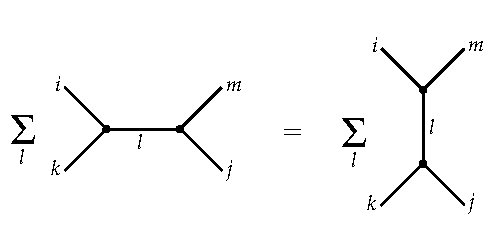
\includegraphics[width=0.8\linewidth]{figures/fig_2_8.pdf}
\caption{OPE の結合則の模式図。}
\label{fig:2.8}
\end{figure}

\subsubsectionlink*{Virasoro 代数と最高ウェイト状態}

今度は Virasoro 生成子について、図\ref{fig:2.6}の議論を考える：
\begin{equation}
\begin{aligned}
L_m\lvert\mathcal A\rangle
&\cong\oint\frac{dz}{2\pi i}\,
z^{m+1}T(z)\mathcal A(0,0)\\
&\cong L_m\cdot\mathcal A(0,0).
\end{aligned}
\tag{2.9.4}\label{eq:2.9.4}
\end{equation}
ここでは新しい考え方と記法を導入した。状態と演算子の同型対応により、Hilbert 空間に作用するすべての演算子には、局所演算子の空間に作用する像がある。言い換えれば、演算子を囲む対応する積分路を取り、その結果生じる局所演算子を OPE で評価するのである。状態を状態に写す $L_m$ に対応するのが、局所演算子を局所演算子に写す $L_m\cdot$ である。一般にはさまざまな位置 $z_i$ に局所演算子があり、各演算子の位置を中心に Laurent 展開して得られる、それぞれ別の Virasoro 代数の複製が存在する。幾何形状によっては、円筒における $z=0$ を中心としたもののように、標準的な生成子の組も存在する。「$\cdot$」は、その特定の演算子の周りの Laurent 係数を論じていることを思い出させるための記号である。

この記法では、$T\mathcal A$ の OPE は
\begin{equation}
T(z)\mathcal A(0,0)=\sum_{m=-\infty}^\infty
z^{-m-2}L_m\cdot\mathcal A(0,0).
\tag{2.9.5}\label{eq:2.9.5}
\end{equation}
以前の記法 \hyperref[eq:2.4.11]{(2.4.11)} との関係は、$n\geq0$ に対して $\mathcal A^{(n)}=L_{n-1}\cdot\mathcal A$ であり、$\mathcal A$ の共形変換は
\begin{equation}
\delta\mathcal A(z,\bar z)
=-\epsilon\sum_{n=0}^\infty\frac1{n!}
\left[\partial^nv(z)L_{n-1}
+(\partial^nv(z))^*\widetilde L_{n-1}\right]\cdot\mathcal A(z,\bar z).
\tag{2.9.6}\label{eq:2.9.6}
\end{equation}
$T\mathcal A$ の OPE の一般形 \hyperref[eq:2.4.14]{(2.4.14)} を使うと、きわめて便利な結果
\begin{align}
L_{-1}\cdot\mathcal A&=\partial\mathcal A,\qquad
\widetilde L_{-1}\cdot\mathcal A=\bar\partial\mathcal A,
\tag{2.9.7a}\label{eq:2.9.7a}\\
L_0\cdot\mathcal A&=h\mathcal A,\qquad
\widetilde L_0\cdot\mathcal A=\widetilde h\mathcal A
\tag{2.9.7b}\label{eq:2.9.7b}
\end{align}
を得る。

OPE \hyperref[eq:2.9.5]{(2.9.5)} より、ウェイト $(h,\widetilde h)$ の一次場 $\mathcal O$ は、
\begin{align}
L_0\lvert\mathcal O\rangle&=h\lvert\mathcal O\rangle,\qquad
\widetilde L_0\lvert\mathcal O\rangle=\widetilde h\lvert\mathcal O\rangle,
\tag{2.9.8a}\label{eq:2.9.8a}\\
L_m\lvert\mathcal O\rangle&=\widetilde L_m\lvert\mathcal O\rangle=0,
\qquad m>0
\tag{2.9.8b}\label{eq:2.9.8b}
\end{align}
を満たす状態に対応する。このような状態は慣例として最高ウェイト状態と呼ばれる。ここで関心のある CFT では、$L_0$ と $\widetilde L_0$ は下に有界である。任意の状態に下降演算子を繰り返し作用させると、ついにはそれ以上の下降演算子によって消滅する状態、すなわち最高ウェイト状態に達する。

興味深い特別な場合は単位演算子である。演算子積 $T1$ には特異性がないため、どの CFT でも
\begin{equation}
L_m\lvert1\rangle=\widetilde L_m\lvert1\rangle=0,
\qquad m\geq-1
\tag{2.9.9}\label{eq:2.9.9}
\end{equation}
が従う。第2.6節で述べたように、演算子 $L_0$ と $L_{\pm1}$ は閉じた代数をなし、$\widetilde L_0$ と $\widetilde L_{\pm1}$ も同様である。全体の代数は
\begin{equation}
SL(2,\mathbb C).
\tag{2.9.10}\label{eq:2.9.10}
\end{equation}
したがって、$\lvert1\rangle$ は $SL(2,\mathbb C)$ 不変状態とも呼ばれる。このような状態はこれだけである。関係 \hyperref[eq:2.9.7a]{(2.9.7)} より、任意の $SL(2,\mathbb C)$ 不変状態に対応する演算子 $\mathcal A$ は位置に依存しないからである。すると、式 \hyperref[eq:2.4.24]{(2.4.24)} の後で説明したように、それは c 数でなければならない。

\subsubsectionlink*{ユニタリーな CFT}

最高ウェイト状態は、弦理論でも Virasoro 代数の表現論でも特別な役割を果たす。これには各所で立ち戻るが、ここではまず、ユニタリーな CFT で成り立つ重要な一般的結果をいくつか導こう。ユニタリーな CFT とは、
\begin{equation}
L_m^\dagger=L_{-m},\qquad
\widetilde L_m^\dagger=\widetilde L_{-m}
\tag{2.9.11}\label{eq:2.9.11}
\end{equation}
を満たす正定値の内積 $\langle\,|\,\rangle$ を持つものである。内積が $\langle\alpha|A\beta\rangle=\langle A^\dagger\alpha|\beta\rangle$ によって随伴を定義することを思い出そう。

たとえば、空間的な $\mu$ については、基底状態の内積を
\begin{equation}
\langle0;k|0;k'\rangle=2\pi\delta(k-k')
\tag{2.9.12}\label{eq:2.9.12}
\end{equation}
と取り、
\begin{equation}
\alpha_m^\dagger=\alpha_{-m},\qquad
\widetilde\alpha_m^\dagger=\widetilde\alpha_{-m}
\tag{2.9.13}\label{eq:2.9.13}
\end{equation}
と定義すれば、$X^\mu$ CFT はユニタリーである。これにより、すべての高い状態の内積も暗黙に定義される。$\mu=0$ では交換子の符号が逆なので、この CFT はユニタリーではない。

第1の制約は、ユニタリーな CFT のどの状態も $h,\widetilde h\geq0$ を持たなければならないことである。これが最高ウェイト状態について正しければ、すべての状態について正しい。最高ウェイト状態には Virasoro 代数から
\begin{equation}
\begin{aligned}
2h_{\mathcal O}\langle\mathcal O|\mathcal O\rangle
&=2\langle\mathcal O|L_0|\mathcal O\rangle
=\langle\mathcal O|[L_1,L_{-1}]|\mathcal O\rangle\\
&=\bigl\|L_{-1}\lvert\mathcal O\rangle\bigr\|^2\geq0
\end{aligned}
\tag{2.9.14}\label{eq:2.9.14}
\end{equation}
が成り立つので、$h_{\mathcal O}\geq0$ である。また、$h_{\mathcal O}=\widetilde h_{\mathcal O}=0$ ならば
\begin{equation}
L_{-1}\cdot\mathcal O=\widetilde L_{-1}\cdot\mathcal O=0
\tag{2.9.15}\label{eq:2.9.15}
\end{equation}
が従うので、$\mathcal O$ は位置に依存しない。先に述べたように、すると $\mathcal O$ は c 数でなければならない。すなわち、ユニタリーな CFT でウェイト $(0,0)$ を持つ演算子は単位演算子だけである。興味深いことに、$X^\mu$ 自身が一つの顕著な例外となる。対応する状態 $x^\mu\lvert0;0\rangle$ は、$X^\mu$ の値域が無限であるため規格化できず、式 \hyperref[eq:2.9.14]{(2.9.14)} はもはや成り立たない。一般定理が最も役立つのは、こうした例外の起こり得ない、コンパクト化された次元に対応する CFT である。

同様に、ユニタリーな CFT の演算子が正則であることは $\widetilde h=0$ と同値であり、反正則であることは $h=0$ と同値であると分かる。重要な結果なので、繰り返しておく：
\begin{equation}
\partial\mathcal A=0\ \Longleftrightarrow\ h=0,\qquad
\bar\partial\mathcal A=0\ \Longleftrightarrow\ \widetilde h=0.
\tag{2.9.16}\label{eq:2.9.16}
\end{equation}
最後に、上の議論で交換子 $[L_n,L_{-n}]$ を用いれば、ユニタリーな CFT では $c,\widetilde c\geq0$ であることを示せる。実際、$c=0$ のユニタリーな CFT は、自明なもの $L_n=0$ しかない。

\subsubsectionlink*{零点エネルギー}

状態と演算子の写像は、さまざまな正規順序定数について別の簡単な導出を与える。どの CFT でも $L_0\lvert1\rangle=0$ であると分かっており、これが $L_0$ の加法的な規格化を決める。$X$ CFT では、$\lvert1\rangle$ は基底状態 $\lvert0;0\rangle$ なので、$a^X$ はゼロになる。$bc$ 理論では $\lvert1\rangle$ は励起状態 $b_{-1}\lvert\downarrow\rangle$ なので、$\lvert\downarrow\rangle$ のウェイトは $-1$ であり、$\lambda=2$ に対する以前の結果 \hyperref[eq:2.7.21]{(2.7.21)} と一致する。

これは中心電荷の物理的解釈の一つも与える。ユニタリーな CFT では基底状態は $\lvert1\rangle$ であり、$L_0=\widetilde L_0=0$ である。すると、動径方向と時間並進の生成子を結ぶ共形変換 \hyperref[eq:2.6.10]{(2.6.10)} より、基底状態について
\begin{equation}
E=-\frac{c+\widetilde c}{24}
\tag{2.9.17}\label{eq:2.9.17}
\end{equation}
が従う。これは系の有限な大きさから生じる Casimir エネルギーであり、中心電荷だけに依存する。次元解析によれば、このエネルギーは系の大きさ $\ell$ に反比例する。ここでは $\ell=2\pi$ なので、一般的な結果は
\begin{equation}
E=-\frac{\pi(c+\widetilde c)}{12\ell}
\tag{2.9.18}\label{eq:2.9.18}
\end{equation}
となる。

これで正規順序定数を計算する正当な方法を三つ与えた。式 \hyperref[eq:2.7.8]{(2.7.8)} のように Virasoro 代数から求める方法、式 \hyperref[eq:2.7.11]{(2.7.11)} のように二種類の正規順序を関係付ける方法、そして上の状態と演算子の写像を用いる方法である。それでも、零点エネルギーを足し合わせる考え方は直観的で、便利な記憶法でもある。そこで、より正当な方法のいずれかで確認できる処方を示す：
\begin{enumerate}
\item 零点エネルギーを足し合わせる。各ボース的モードには $\frac12\omega$、各フェルミ的（反交換する）モードには $-\frac12\omega$ を割り当てる。
\item $\sum_{n=1}^\infty(n-\theta)$ の形の発散する和が現れる。$\theta$ は非自明な周期条件を考えるときに生じる。これを
\begin{equation}
\sum_{n=1}^\infty(n-\theta)=\frac1{24}-\frac18(2\theta-1)^2
\tag{2.9.19}\label{eq:2.9.19}
\end{equation}
と定義する。これは式 \hyperref[eq:1.3.32]{(1.3.32)} と同じく、正則化して2次発散部分を捨てると得られる値である。
\item 以上で得られるのは、$w$ 座標系の生成子 $T_0$、式 \hyperref[eq:2.6.8]{(2.6.8)}、の正規順序定数である。$L_0$ については、テンソル的でない補正 $\frac1{24}c$ を加えなければならない。
\end{enumerate}
自由ボソンではモードは整数値なので、手順2の後には $\theta=0$ に対する和 \hyperref[eq:2.9.19]{(2.9.19)} の半分、すなわち $-\frac1{24}$ が得られる。これは手順3の補正でちょうど相殺され、$a^X=0$ となる。ゴーストについても同様に、$\frac2{24}-\frac{26}{24}=-1$ を得る。

\subsectionlink*{演習}
\addcontentsline{toc}{subsection}{演習問題}
\label{sec:2.exercises}
\providecommand{\bndnorm}[1]{\mathopen{{}^{\star}_{\star}}#1\mathclose{{}^{\star}_{\star}}}

\subsubsection*{演習2.1}\label{ex:2.1}
\[
\partial\bar\partial\ln|z|^2
=\partial\frac1{\bar z}
=\bar\partial\frac1z
=2\pi\delta^2(z,\bar z)
\]
を次の方法で確認せよ。

\noindent
(a) 発散定理 \hyperref[eq:2.1.9]{(2.1.9)} を用いる。

\noindent
(b) 特異性を正則化してから極限を取る。

\medskip
\subsubsection*{演習2.2}\label{ex:2.2}
四つの場 $X^\mu$ の正規順序積について、式 \hyperref[eq:2.2.5]{(2.2.5)} を明示的に書き下せ。それが各位置について調和関数であることを示せ。

\medskip
\subsubsection*{演習2.3}\label{ex:2.3}
平面上での指数演算子の積の期待値は
\[
\left\langle\prod_{i=1}^n:e^{ik_i\cdot X(z_i,\bar z_i)}:\right\rangle
=iC^X(2\pi)^D\delta^D\left(\sum_{i=1}^n k_i\right)
\prod_{\substack{i,j=1\\i<j}}^n|z_{ij}|^{\alpha'k_i\cdot k_j},
\]
であり、$C^X$ は定数である。これは、第6章でいくつかの方法により求める球面上の期待値 (6.2.17) の極限として得られる。

\noindent
(a) 一つの頂点演算子が別の頂点演算子に近づくときの主要な振る舞いが、OPE \hyperref[eq:2.2.14]{(2.2.14)} と一致することを示せ。

\noindent
(b) 式 \hyperref[eq:2.2.13]{(2.2.13)} が示すように、期待値は、$z_1\to z_2$ で滑らかな関数に $|z_{12}|^{\alpha'k_1\cdot k_2}$ を掛けたものである。$n=3$ について、この滑らかな関数を $z_{12}$ と $\bar z_{12}$ のべきで明示的に展開せよ。高次の項の比から収束半径を求めよ。

\noindent
(c) 自由場の OPE \hyperref[eq:2.2.4]{(2.2.4)} が図\ref{fig:2.1}の破線の円の内部で収束することの一般的な証明を与えよ。

\medskip
\subsubsection*{演習2.4}\label{ex:2.4}
OPE \hyperref[eq:2.2.14]{(2.2.14)} を、$z^2$、$z\bar z$、$\bar z^2$ の次数の劣主要項まで含めて拡張せよ。各項の $z,\bar z$ 依存性が一般形 \hyperref[eq:2.4.20]{(2.4.20)} と一致することを示せ。また、式 \hyperref[eq:2.2.15]{(2.2.15)} のような対称な形を与え、二つの演算子の交換に対する係数の性質を論じよ。

\medskip
\subsubsection*{演習2.5}\label{ex:2.5}
教科書で通常見られる形の古典的 Noether の定理を導け。すなわち、
\[
S[\phi]=\int d^d\sigma\,
\mathcal L\bigl(\phi(\sigma),\partial_a\phi(\sigma)\bigr)
\]
と仮定し、測度の変分は無視せよ。作用の不変性は、対称変換 \hyperref[eq:2.3.1]{(2.3.1)} の下で Lagrangian 密度の変分が全微分、
\[
\delta\mathcal L=\epsilon\partial_a\mathcal K^a
\]
となることを意味する。このとき、弦で慣用される規格化を用いた古典的な結果は
\[
j^a=2\pi i\left(
\frac{\partial\mathcal L}{\partial\phi_{\alpha,a}}\,
\epsilon^{-1}\delta\phi_\alpha-\mathcal K^a\right)
\]
である。Lagrange の運動方程式を導き、そこからこのカレントが保存されることを示せ。また、これが式 \hyperref[eq:2.3.4]{(2.3.4)} と一致することを示せ。

\medskip
\subsubsection*{演習2.6}\label{ex:2.6}
$d$ 次元の平坦な Euclid 計量 $\delta_{ab}$ を考える。無限小座標変換 $\delta\sigma^a=v^a(\sigma)$ は、計量を $\delta g_{ab}=-\partial_av_b-\partial_bv_a$ だけ変化させる。局所的なスケール変換を除いて計量を不変に保つ、最も一般的な $v^a(\sigma)$ を決定せよ。$d>2$ では独立な解が $\frac12(d+1)(d+2)$ 個あり、$d=2$ では無限個ある。［結果は文献の多くの場所に与えられているが、著者は簡単な導出を見いだしていない。］

\medskip
\subsubsection*{演習2.7}\label{ex:2.7}
(a) 関係する OPE を計算し、式 \hyperref[eq:2.4.17]{(2.4.17)} に記されたウェイトを確認するとともに、どの演算子がテンソルであるかを決定せよ。

\noindent
(b) 線形ディラトン理論における同じ演算子について、同じことを行え。

\medskip
\subsubsection*{演習2.8}\label{ex:2.8}
$f_{\mu\nu}:\partial X^\mu\bar\partial X^\nu e^{ik\cdot X}:$ のウェイトはいくらか。これがテンソルとなるための $f_{\mu\nu}$ と $k_\mu$ に対する条件は何か。

\medskip
\subsubsection*{演習2.9}\label{ex:2.9}
$TT$ の OPE を求めて、線形ディラトン、$bc$、$\beta\gamma$ の各 CFT の中心電荷を導け。

\medskip
\subsubsection*{演習2.10}\label{ex:2.10}
今度は境界を持つ世界面の一部分を考える。便宜上、その領域は $z$ 上半平面内にあり、実軸が境界であるとする。正規順序演算子、たとえば $:\partial X^\mu(z)\bar\partial X_\mu(\bar z):$ の期待値は、内部では有限であっても、$z$ が境界に近づくと発散することを示せ（境界の効果を鏡像電荷で表せ）。縮約に鏡像電荷の部分も含める点を除いて $:\ :$ と同じである、境界正規順序 $\bndnorm{\phantom X}$ を定義せよ。境界上の演算子は、境界正規順序にすれば有限である。

境界を持つ多様体上の一般の CFT では、内部の演算子と境界の演算子は独立である。それぞれの基底を $\mathcal A_i$ と $\mathcal B_r$ でラベル付けし、前者を $:\ :$、後者を $\bndnorm{\phantom X}$ によって定義する。各集合はそれぞれ閉じた OPE、$\mathcal A\mathcal A\to\mathcal A$ および $\mathcal B\mathcal B\to\mathcal B$、を持つ。さらに、これらの集合は互いに関係している。$\mathcal A_i$ は境界に近づくと、$\mathcal B_r$ で展開できる。次の主要な振る舞いを求めよ：
\[
\begin{aligned}
&\bndnorm{e^{ik_1\cdot X(y_1)}}\,
\bndnorm{e^{ik_2\cdot X(y_2)}},
&&y_1\to y_2\quad(y\text{ は実数}),\\
&:e^{ik\cdot X(z,\bar z)}:,
&&\operatorname{Im}z\to0.
\end{aligned}
\]
後者には恒等式 \hyperref[eq:2.7.14]{(2.7.14)} が有用である。

\medskip
\subsubsection*{演習2.11}\label{ex:2.11}
\[
L_m(L_{-m}\lvert0;0\rangle)
-L_{-m}(L_m\lvert0;0\rangle)
\]
を計算し、$X^\mu$ に対する Virasoro 代数の中心電荷を評価せよ。

\medskip
\subsubsection*{演習2.12}\label{ex:2.12}
OPE と積分路の結果 \hyperref[eq:2.6.14]{(2.6.14)}、\hyperref[eq:2.6.15]{(2.6.15)} を用いて、交換関係 \hyperref[eq:2.7.5a]{(2.7.5)} と \hyperref[eq:2.7.17]{(2.7.17)} を導け。

\medskip
\subsubsection*{演習2.13}\label{ex:2.13}
(a) 式 \hyperref[eq:2.7.11]{(2.7.11)} の方法で、
\[
:b(z)c(z'):-\canorm{b(z)c(z')}
=\frac{(z/z')^{1-\lambda}-1}{z-z'}
\]
を示せ。

\noindent
(b) これを用いて、$N^{\mathrm g}$、式 \hyperref[eq:2.7.22]{(2.7.22)}、の順序定数を決定せよ。共形変換 \hyperref[eq:2.8.14]{(2.8.14)} も必要である。

\noindent
(c) 第2.9節と同様の、順序に関する発見的な取り扱いからも、$N^{\mathrm g}$ の同じ値が得られることを示せ。

\medskip
\subsubsection*{演習2.14}\label{ex:2.14}
(a) 前の演習の (a) を用いて、$L_0^{\mathrm g}$、式 \hyperref[eq:2.7.21]{(2.7.21)}、の順序定数を決定せよ。

\noindent
(b) 第2.9節の発見的な規則を用いて、それを決定せよ。

\medskip
\subsubsection*{演習2.15}\label{ex:2.15}
開弦の $X^\mu$ CFT について、状態と演算子の写像を求めよ。

\medskip
\subsubsection*{演習2.16}\label{ex:2.16}
$\mathcal O$ をウェイト $(h,\widetilde h)$ のテンソル場とする。図\ref{fig:2.4}の積分路の議論を用いて交換子 $[L_m,\mathcal O(z,\bar z)]$ を評価せよ。とくに、$(1,1)$ テンソルの交換子が全微分であることを示せ。

\medskip
\subsubsection*{演習2.17}\label{ex:2.17}
式 \hyperref[eq:2.9.14]{(2.9.14)} の議論を拡張し、$c\geq0$ を示せ。
